\subsection*{Report 4}

In figure \ref{figure:2_2} the train signal is reshaped into segments of 20ms, and afterwards the DFT is applied to each segment. Enlarging the segment size will give a better resolution on the frequency axis, but lower on the time axis. The opposite is also true: smaller segment size gives a better time resolution, but worse frequency resolution. This plot is more useful than the non-segmented plot in figure \ref{figure:2_1} since variations in time in the signal are now visible.
	\begin{figure}[H] 
		\centering
		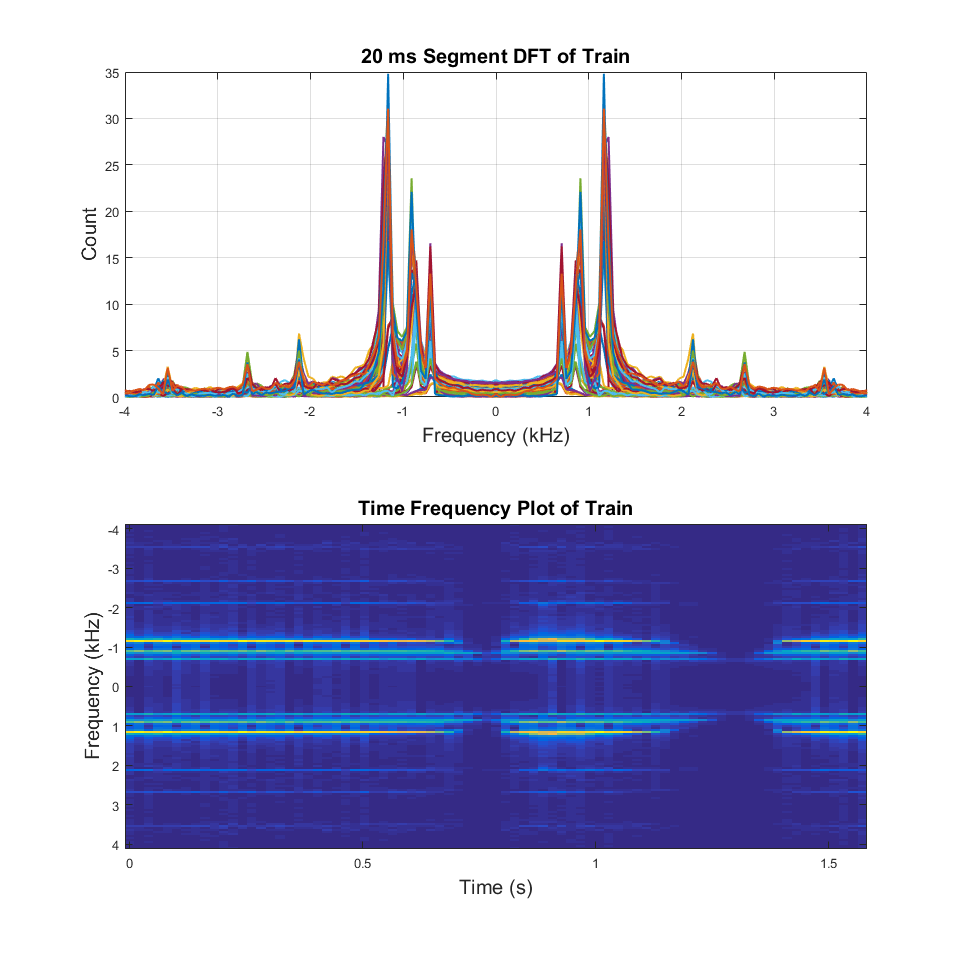
\includegraphics[width=\textwidth]{2.2.png}
		\caption{Train - Segmented FFT \& Time Frequency Plot}
		\label{figure:2_2}
	\end{figure}
	
	